\section{Aufbau und Durchführung}
\begin{figure}[H]
  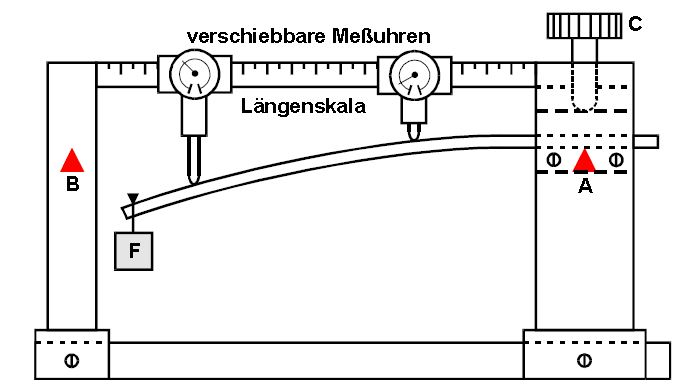
\includegraphics[width=\textwidth]{Text/Bilder/Aufbau.png}
  \caption{Aufbau \cite[3]{sample1}}
  \label{fig:Aufbau}
\end{figure}
Zunächst wird der in Abbildung \ref{fig:Aufbau} zu sehende Aufbau aufgebaut und die Apparatur auf "COOL" gestellt.
Ebenso wird der Abstand zwischen den Thermoelementen gemessen.
Daraufhin wird kontrolliert, ob der Temperatur-Array alle Sensoren erkennt und die Abtastrate auf $\SI{5}{\s}$ eingestellt.
Die Isolierungen werden auf die Stäbe gelegt und die Apparatur auf "HEAT" gestellt. Sobald T7 eine Temperatur von
$\SI{45}{\celsius}$ erreicht, wird die Messung beendet und die Isolierungen entfernt.
Nachdem alle Stäbe auf eine Temperatur von $\SI{30}{\celsius}$ oder weniger abgekühlt sind, beginnt eine zweite Messreihe.
In dieser werden die Metalle über 10 Perioden erhitzt. Dabei wird die Apparatur in einer Periode $\SI{40}{\s}$ auf "HEAT"
und $\SI{40}{\s}$ auf "COOL" gestellt. Die Abtastrate wird dabei auf $\SI{2}{\s}$ gestellt.
Erreicht ein Metall eine Temperatur von $\SI{80}{\celsius}$ bevor die 10 Perioden abgeschlossen sind, wird die Messung beendet.
Ist diese Messung abgeschlossen, wird sie wiederholt. Jedoch mit dem Unterschied, dass die Apparatur in einer Periode
nun $\SI{200}{\s}$ auf "HEAT" und $\SI{200}{\s}$ auf "COOL" gestellt wird.
